\documentclass{article}
\usepackage[a4paper,margin=1in]{geometry}
\usepackage[utf8]{inputenc}
\usepackage{graphicx}
\graphicspath{ {./images/} }
\title{\Large Brick game: Tetris. Documentation}
\author{SIONAPAE}
\date{05.10.24}

\begin{document}
\maketitle

\begin{figure}[h]
\end{figure}
\section{Project Description}
Implementation of the "Tetris" game in C using a structured approach.

\section{Requirements}
To run the program, you need:
\begin{itemize}
    \item GCC compiler or any other C++-compatible compiler
    \item GNU Make to build the program
    \item The libraries check.h and ncurses.h
\end{itemize}

\section{How to Build and Run the Game}
\begin{enumerate}
    \item Run the command `make all` to build the program.
    \item Start the game by running `make run`.
    \begin{itemize}
        \item all  
        \item install — compiles the Tetris source file
        \item run — runs the game 
        \item uninstall — deletes the Tetris executable 
        \item clean — removes build files
        \item dvi — project documentation
        \item dist — archives the project 
        \item test — runs unit tests 
        \item gcov\_report — generates an HTML coverage report
    \end{itemize}
\end{enumerate}

\section{Controls}
The player uses keyboard keys that simulate physical buttons on a real console to control falling blocks:
\begin{itemize}
    \item D key — Left arrow — move the block left.
    \item A key — Right arrow — move the block right.
    \item F key — Down arrow — make the block fall.
    \item S key — accelerates the fall of the block.
    \item W key — Up arrow — rotate the block.
    \item P/SPACE key — pause the game.
    \item N/ENTER key — start a new game or continue.
    \item q/ESCAPE key — quit the current game, exit the application.
\end{itemize}

\section{Program Architecture}
A finite state machine for a specific implementation of the Tetris game.

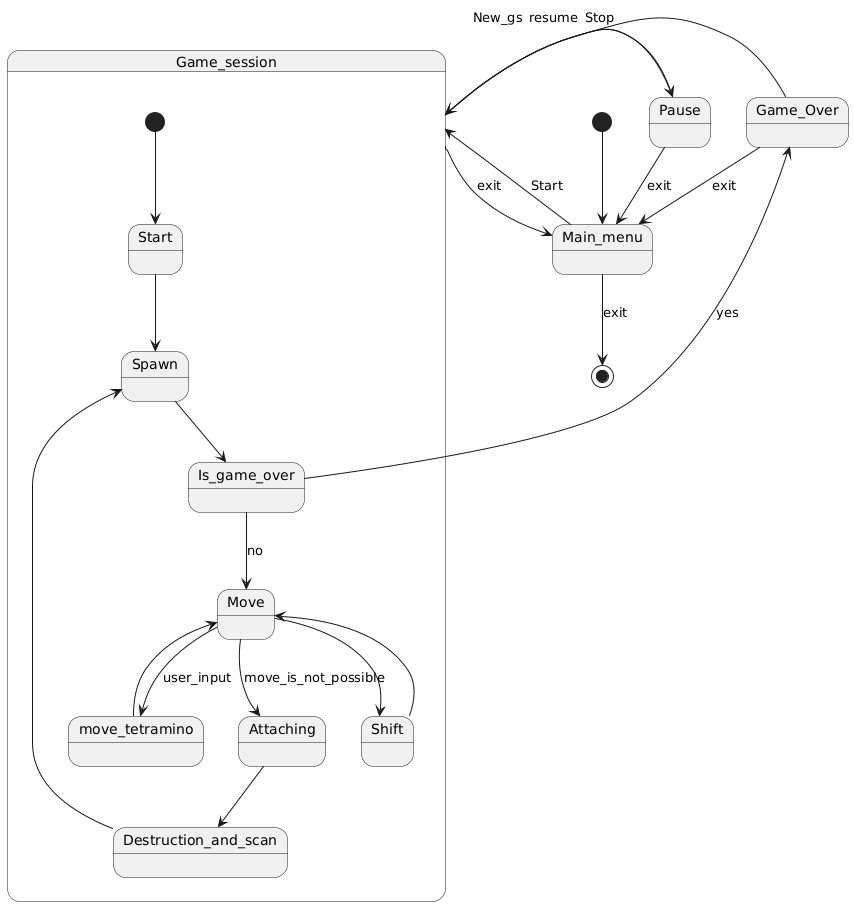
\includegraphics[width=10cm, height=10cm]{images/FSM.png}

The program is built around a Finite State Machine (FSM) that manages the game’s logic. The \texttt{main()} function sets up the environment, starts the game loop via \texttt{game\_loop()}, and handles game termination.

The entire code structure is organized as follows:

\subsection{\texttt{main()}: Entry Point}

This function initializes the game environment, runs the main game loop, and cleans up when the game finishes.

\begin{itemize}
    \item \textbf{Random number generator initialization:}
    \begin{verbatim}
    srand(time(0));
    get_random();
    \end{verbatim}
    Here, the random number generator is initialized to generate random Tetrimino pieces.
    
    \item \textbf{Game objects initialization:}
    \begin{verbatim}
    Game_Objects_t* params = get_instanse();
    *params = init_empty_game_objects();
    \end{verbatim}
    The \texttt{params} object holds information about the current game state, user actions, and game objects.

    \item \textbf{Ncurses initialization and game loop start:}
    \begin{verbatim}
    #ifndef debug_bro
    init_bro_ncurses(&params->views);
    game_loop();
    terminate_ncurses_bro(&params->views);
    #else
    game_loop();
    #endif
    \end{verbatim}
    Depending on the compilation mode, the game either uses ncurses for a console user interface (CUI) or runs in debug mode without ncurses.
\end{itemize}

\subsection{\texttt{game\_loop()}: The Main Game Loop}

The \texttt{game\_loop()} function runs until the game is over. It processes the main game states and user actions.

\begin{itemize}
    \item \textbf{Game state initialization:}
    \begin{verbatim}
    State prev = START;
    \end{verbatim}
    The variable \texttt{prev} stores the previous state of the game to return to it after pause or other states.

    \item \textbf{Main game loop:}
    \begin{verbatim}
    while (params->game_is_running) {
        draw_static(params);
        main_game_fsm(params);
        game_session(params, &prev);
    }
    \end{verbatim}
    The main loop continues as long as \texttt{game\_is\_running == true}. It processes game states and user actions within the loop.
\end{itemize}

\subsection{\texttt{game\_session()}: Managing the Game Session}

The \texttt{game\_session()} function controls the actual gameplay (such as moving the Tetriminos, counting time, and handling pauses).

\begin{itemize}
    \item \textbf{Game session initialization:}
    \begin{verbatim}
    if (params->state == START) {
        session_is_running = true;
        params->state = *prev;
    }
    \end{verbatim}
    If the game begins in the \texttt{START} state, the previous game state is restored, and a new game session starts.

    \item \textbf{Game session loop:}
    \begin{verbatim}
    while (params->state != PAUSE && params->state != GAME_OVER && params->state != MAIN_MENU) {
        fsm_game_session(params);
        key = getch();
        userInput(getSignal(key), session_is_running);
        countTime(params);
    }
    \end{verbatim}
    The loop continues until the game ends (GAME\_OVER) or is paused. Inside the loop, user actions (move, pause, quit) are processed, and the game state is updated.
    
    \item \textbf{Saving high scores:}
    \begin{verbatim}
    if (params->gameInfo.score > params->gameInfo.high_score)
        write_high_score(params->gameInfo.score);
    \end{verbatim}
    If the player achieves a new high score, it is saved.
\end{itemize}

\section{Technologies and Libraries Used}

\begin{itemize}
    \item \textbf{Compiler version:} Recommended version — GCC 9.3
    \item \textbf{External libraries:}
    \begin{itemize}
        \item \texttt{ncurses.h} — library for working with console user interfaces (CUI). It provides functions for terminal control, input processing, and window management in text mode.
    \end{itemize}
\end{itemize}

\end{document}
